\documentclass{standalone}
\usepackage{graphicx}	
\usepackage{amssymb, amsmath, amsthm}
\usepackage{color}

\usepackage{tikz}
\usetikzlibrary{intersections, backgrounds}

\definecolor{light}{RGB}{220, 188, 188}
\definecolor{mid}{RGB}{185, 124, 124}
\definecolor{dark}{RGB}{143, 39, 39}
\definecolor{highlight}{RGB}{180, 31, 180}
\definecolor{gray10}{gray}{0.1}
\definecolor{gray20}{gray}{0.2}
\definecolor{gray30}{gray}{0.3}
\definecolor{gray40}{gray}{0.4}
\definecolor{gray60}{gray}{0.6}
\definecolor{gray70}{gray}{0.7}
\definecolor{gray80}{gray}{0.8}
\definecolor{gray90}{gray}{0.9}
\definecolor{gray95}{gray}{0.95}

\begin{document}

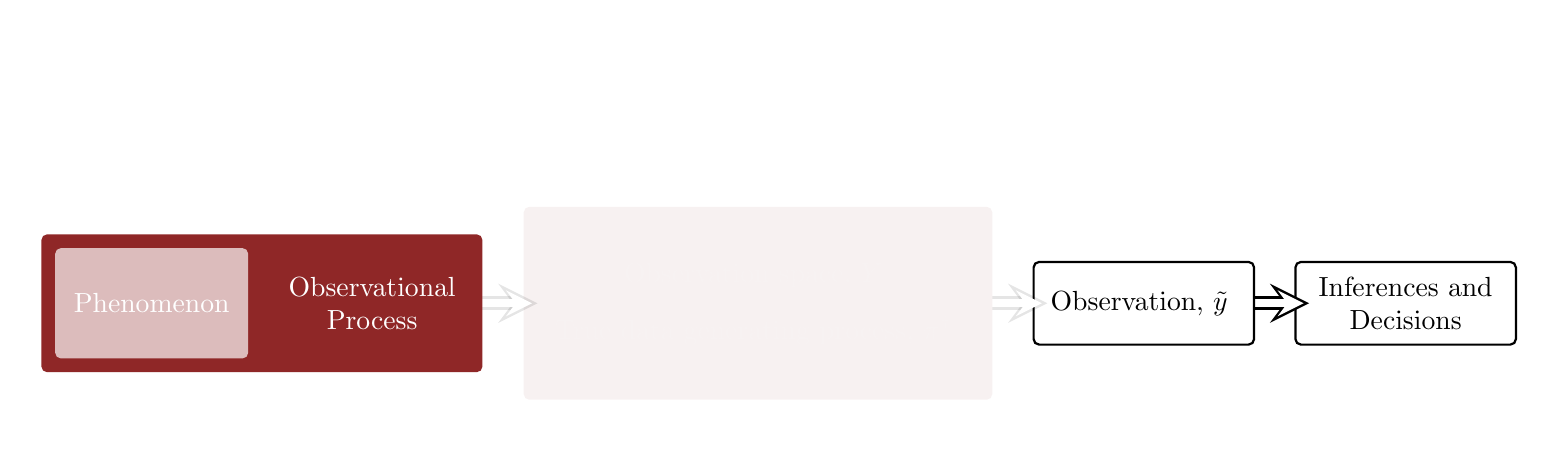
\begin{tikzpicture}[scale=0.35, thick]
  \fill [white] (-8.5, -5) rectangle +(54, 15);

  \fill [rounded corners=2pt, color=white] (37.5, -1.5) rectangle +(8, 3);
  \draw [rounded corners=2pt] (37.5, -1.5) rectangle +(8, 3)
  node[midway, align=center] { Inferences and\\Decisions }; 
  
  \draw[->, >=stealth, line width=5] (36, 0) -- (38, 0);
  \draw[->, >=stealth, line width=3, white] (36, 0) -- (37.8, 0);
  
  \draw [rounded corners=2pt] (28, -1.5) rectangle +(8, 3) 
  node[midway, align=center] { Observation, $\tilde{y}$ }; 
  
  \draw[->, >=stealth, line width=5, opacity=0.10] (25.5, 0) -- (28.5, 0);
  \draw[->, >=stealth, line width=3, white] (25.5, 0) -- (28.3, 0);
  
  \fill [rounded corners=2pt, fill=white] (9.5, -3.5) rectangle +(17, 7);
  \fill [rounded corners=2pt, fill=mid, text=white, opacity=0.10] (9.5, -3.5) rectangle +(17, 7) 
  node[midway, yshift=10, align=center] { Observation space, $Y$ }
  node[midway, yshift=-10, align=center] { True data generating process, $\pi^{\dagger}$ };

  \draw[->, >=stealth, line width=5, opacity=0.10] (8, 0) -- (10, 0);
  \draw[->, >=stealth, line width=3, white] (8, 0) -- (9.8, 0);

  \fill [rounded corners=2pt, color=dark, dashed] (-8, -2.5) rectangle +(16, 5);
  \node at (4, 0) [text=white, align=center] {Observational\\Process};
  
  \fill [rounded corners=2pt, fill=light, text=white] (-7.5, -2) rectangle +(7, 4) 
  node [midway, align=center] {Phenomenon};
  
\end{tikzpicture}

\end{document}  